\documentclass[12pt]{article}
\usepackage[x11names, svgnames, rgb]{xcolor}
\usepackage{amsmath}
\usepackage{amssymb}
\usepackage{geometry}
\usepackage{setspace}
\usepackage{pgfplots}
\usepackage{tikz}
\usetikzlibrary{snakes,arrows,shapes}

\setlength{\parskip}{1em}
\geometry{
	a4paper,
	total={170mm,257mm},
	left=20mm,
	top=20mm,
}

\title{}
\author{}
\date{}

\begin{document}
\maketitle
\vspace{-5cm}
\noindent
\textbf{Exercise 1.14:} Draw the tree illustrating the process generated by the
\verb|count-change| procedure of Section 1.2.2 in making change for 11 cents.
What are the orders of growth of the space and number of steps used by this process as
the amount to be changed increases? \\

\textbf{Ans.} The procedure tree for \verb|(cc 11 5)| is presented below:

\scalebox{0.5}{
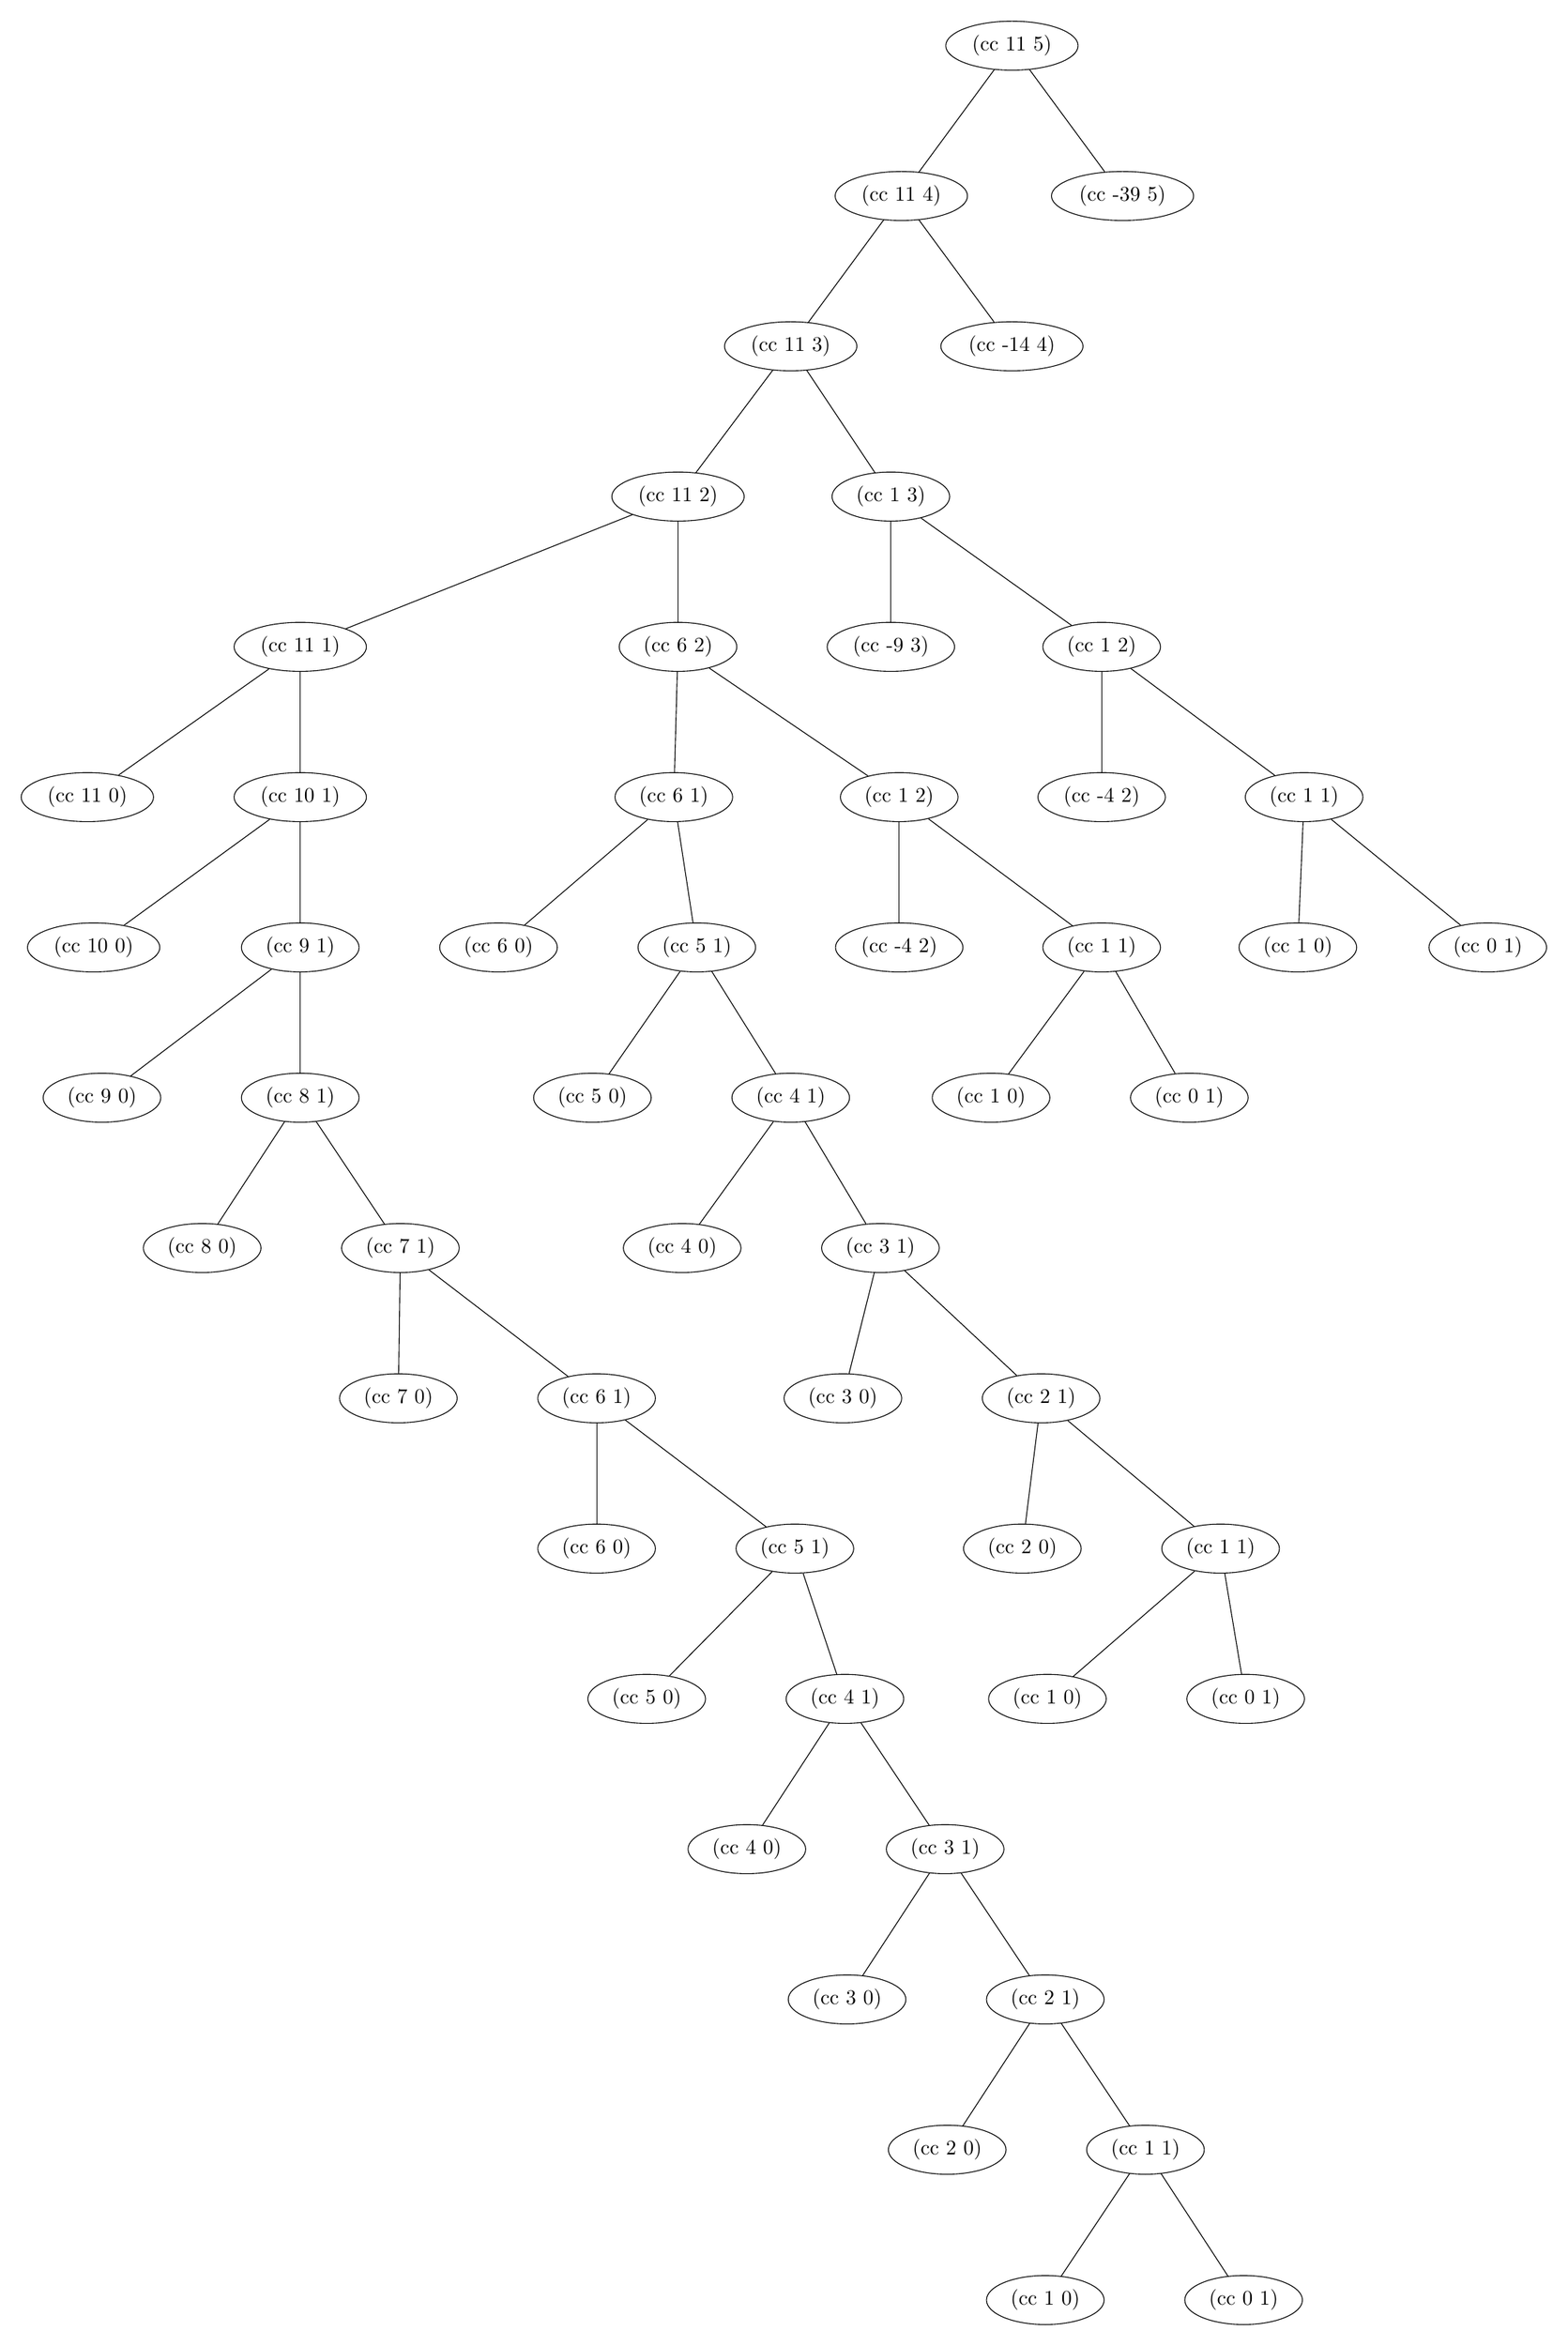
\begin{tikzpicture}[>=latex',line join=bevel,] %I've used dot2tex for that
%%
\node (1) at (485.25bp,1098.0bp) [draw,ellipse] {(cc 11 5)};
  \node (2) at (432.25bp,1026.0bp) [draw,ellipse] {(cc 11 4)};
  \node (3) at (538.25bp,1026.0bp) [draw,ellipse] {(cc -39 5)};
  \node (4) at (379.25bp,954.0bp) [draw,ellipse] {(cc 11 3)};
  \node (5) at (485.25bp,954.0bp) [draw,ellipse] {(cc -14 4)};
  \node (6) at (325.25bp,882.0bp) [draw,ellipse] {(cc 11 2)};
  \node (7) at (427.25bp,882.0bp) [draw,ellipse] {(cc 1 3)};
  \node (14) at (144.25bp,810.0bp) [draw,ellipse] {(cc 11 1)};
  \node (15) at (325.25bp,810.0bp) [draw,ellipse] {(cc 6 2)};
  \node (8) at (427.25bp,810.0bp) [draw,ellipse] {(cc -9 3)};
  \node (9) at (528.25bp,810.0bp) [draw,ellipse] {(cc 1 2)};
  \node (10) at (528.25bp,738.0bp) [draw,ellipse] {(cc -4 2)};
  \node (11) at (625.25bp,738.0bp) [draw,ellipse] {(cc 1 1)};
  \node (12) at (622.25bp,666.0bp) [draw,ellipse] {(cc 1 0)};
  \node (13) at (713.25bp,666.0bp) [draw,ellipse] {(cc 0 1)};
  \node (22) at (42.246bp,738.0bp) [draw,ellipse] {(cc 11 0)};
  \node (23) at (144.25bp,738.0bp) [draw,ellipse] {(cc 10 1)};
  \node (16) at (323.25bp,738.0bp) [draw,ellipse] {(cc 6 1)};
  \node (17) at (431.25bp,738.0bp) [draw,ellipse] {(cc 1 2)};
  \node (44) at (239.25bp,666.0bp) [draw,ellipse] {(cc 6 0)};
  \node (45) at (334.25bp,666.0bp) [draw,ellipse] {(cc 5 1)};
  \node (18) at (431.25bp,666.0bp) [draw,ellipse] {(cc -4 2)};
  \node (19) at (528.25bp,666.0bp) [draw,ellipse] {(cc 1 1)};
  \node (20) at (475.25bp,594.0bp) [draw,ellipse] {(cc 1 0)};
  \node (21) at (570.25bp,594.0bp) [draw,ellipse] {(cc 0 1)};
  \node (24) at (45.246bp,666.0bp) [draw,ellipse] {(cc 10 0)};
  \node (25) at (144.25bp,666.0bp) [draw,ellipse] {(cc 9 1)};
  \node (26) at (49.246bp,594.0bp) [draw,ellipse] {(cc 9 0)};
  \node (27) at (144.25bp,594.0bp) [draw,ellipse] {(cc 8 1)};
  \node (28) at (97.246bp,522.0bp) [draw,ellipse] {(cc 8 0)};
  \node (29) at (192.25bp,522.0bp) [draw,ellipse] {(cc 7 1)};
  \node (30) at (191.25bp,450.0bp) [draw,ellipse] {(cc 7 0)};
  \node (31) at (286.25bp,450.0bp) [draw,ellipse] {(cc 6 1)};
  \node (32) at (286.25bp,378.0bp) [draw,ellipse] {(cc 6 0)};
  \node (33) at (381.25bp,378.0bp) [draw,ellipse] {(cc 5 1)};
  \node (34) at (310.25bp,306.0bp) [draw,ellipse] {(cc 5 0)};
  \node (35) at (405.25bp,306.0bp) [draw,ellipse] {(cc 4 1)};
  \node (36) at (358.25bp,234.0bp) [draw,ellipse] {(cc 4 0)};
  \node (37) at (453.25bp,234.0bp) [draw,ellipse] {(cc 3 1)};
  \node (38) at (406.25bp,162.0bp) [draw,ellipse] {(cc 3 0)};
  \node (39) at (501.25bp,162.0bp) [draw,ellipse] {(cc 2 1)};
  \node (40) at (454.25bp,90.0bp) [draw,ellipse] {(cc 2 0)};
  \node (41) at (549.25bp,90.0bp) [draw,ellipse] {(cc 1 1)};
  \node (42) at (501.25bp,18.0bp) [draw,ellipse] {(cc 1 0)};
  \node (43) at (596.25bp,18.0bp) [draw,ellipse] {(cc 0 1)};
  \node (46) at (284.25bp,594.0bp) [draw,ellipse] {(cc 5 0)};
  \node (47) at (379.25bp,594.0bp) [draw,ellipse] {(cc 4 1)};
  \node (48) at (327.25bp,522.0bp) [draw,ellipse] {(cc 4 0)};
  \node (49) at (422.25bp,522.0bp) [draw,ellipse] {(cc 3 1)};
  \node (50) at (404.25bp,450.0bp) [draw,ellipse] {(cc 3 0)};
  \node (51) at (499.25bp,450.0bp) [draw,ellipse] {(cc 2 1)};
  \node (52) at (490.25bp,378.0bp) [draw,ellipse] {(cc 2 0)};
  \node (53) at (585.25bp,378.0bp) [draw,ellipse] {(cc 1 1)};
  \node (54) at (502.25bp,306.0bp) [draw,ellipse] {(cc 1 0)};
  \node (55) at (597.25bp,306.0bp) [draw,ellipse] {(cc 0 1)};
  \draw [] (1) -- (2);
  \draw [] (1) -- (3);
  \draw [] (2) -- (4);
  \draw [] (2) -- (5);
  \draw [] (4) -- (6);
  \draw [] (4) -- (7);
  \draw [] (6) -- (14);
  \draw [] (6) -- (15);
  \draw [] (7) -- (8);
  \draw [] (7) -- (9);
  \draw [] (9) -- (10);
  \draw [] (9) -- (11);
  \draw [] (11) -- (12);
  \draw [] (11) -- (13);
  \draw [] (14) -- (22);
  \draw [] (14) -- (23);
  \draw [] (15) -- (16);
  \draw [] (15) -- (17);
  \draw [] (16) -- (44);
  \draw [] (16) -- (45);
  \draw [] (17) -- (18);
  \draw [] (17) -- (19);
  \draw [] (19) -- (20);
  \draw [] (19) -- (21);
  \draw [] (23) -- (24);
  \draw [] (23) -- (25);
  \draw [] (25) -- (26);
  \draw [] (25) -- (27);
  \draw [] (27) -- (28);
  \draw [] (27) -- (29);
  \draw [] (29) -- (30);
  \draw [] (29) -- (31);
  \draw [] (31) -- (32);
  \draw [] (31) -- (33);
  \draw [] (33) -- (34);
  \draw [] (33) -- (35);
  \draw [] (35) -- (36);
  \draw [] (35) -- (37);
  \draw [] (37) -- (38);
  \draw [] (37) -- (39);
  \draw [] (39) -- (40);
  \draw [] (39) -- (41);
  \draw [] (41) -- (42);
  \draw [] (41) -- (43);
  \draw [] (45) -- (46);
  \draw [] (45) -- (47);
  \draw [] (47) -- (48);
  \draw [] (47) -- (49);
  \draw [] (49) -- (50);
  \draw [] (49) -- (51);
  \draw [] (51) -- (52);
  \draw [] (51) -- (53);
  \draw [] (53) -- (54);
  \draw [] (53) -- (55);
%
\end{tikzpicture}
}

The space complexity of \verb|count-change| corresponds to the longest branch of its
procedure tree. That is, let $n$ be the amount to be changed and $k$ be the argument of
\verb|first-denomination|, denoted by $g(k)$, then the space complexity of \verb|count-change| is $n+k$ or
just $\Theta(n)$.

\newpage

When it comes to the time complexity $T(n,k)$, we first note that for $k=1$, $T(n,1) = 2n-1 = \Theta(n)$.
Then for $k=2$ we may observe that
\begin{align*}
  T(n,2) = 1 + \left\lfloor\frac{n}{5}\right\rfloor + \sum_{i=0}^{\left\lfloor\frac{n}{5}\right\rfloor}T(n-5i, 1) 
\end{align*}
from which we may suspect that $T(n,2) = \Theta(n^2)$ and in general $T(n,k) = \Theta(n^k)$.
This can be turned into a rigorous (?) argument by induction on $k$. We have already considered the
case for $k=1$, so if $T(n,k) = \Theta(n^k)$, then
\begin{align*}
  T(n,k+1) &= 1 + \left\lfloor\frac{n+1}{g(k+1)}\right\rfloor + \sum_{i=0}^{\left\lfloor\frac{n}{g(k+1)}\right\rfloor}T(n-ig(k+1), k) \\
           &= 1 + \Theta(n) + \sum_{i=0}^{\left\lfloor\frac{n}{g(k+1)}\right\rfloor}\Theta((n-ig(k+1))^k) \\
           &= \Theta(n) + \sum_{i=0}^{\left\lfloor\frac{n}{g(k+1)}\right\rfloor}\Theta(n^k) \\
           &= \Theta(n) + \left\lfloor\frac{n}{g(k+1)}\right\rfloor\Theta(n^k) \\
           &= \Theta(n) + \Theta\left(\left\lfloor\frac{n}{g(k+1)}\right\rfloor n^k\right) \\
           &= \Theta(n) + \Theta(n^{k+1}) \\
           &= \Theta(n^{k+1}),
\end{align*}
as desired.

\end{document}

